%--------- Student instruction: change this by adding your neu id into the {}
\def\yourname{patel.nisargs}
%-------------------------------------------------------------------------------------------------------------

%% ================= no need to edit any of this stuff
% --- no need to change anything in this section -----------------------------------------------------
\def\homework{1} % 0 for solution, 1 for problem-set only
\def\duedate{wed feb 9, 2022 at 11.59p}
\def\duelocation{via \href{https://gradescope.com/courses/331917}{gradescope}}
\def\hnumber{2}
\def\prof{abhi shelat}
\def\course{\href{https://shelat.khoury.neu.edu/22s-5800}{cs5800 algorithms s'22}}

\documentclass[11pt]{article}
%%% ==== standard installations of latex include all of the files that are referenced in this section.  However,
%%% ==== if you are having compile problems, consider commenting some of these commands out 
\usepackage[colorlinks,urlcolor=blue]{hyperref}
\usepackage[osf]{mathpazo}
\usepackage{amsmath,amsfonts,graphicx}
\usepackage{latexsym}
\usepackage[top=1in,bottom=1.3in,left=1.5in,right=1.5in,centering]{geometry}
\usepackage{color}
\usepackage{clrscode}
\definecolor{mdb}{rgb}{0.3,0.02,0.02} 
\definecolor{cit}{rgb}{0.05,0.2,0.45} 
\markboth{\yourname}{\yourname}
%%% ===================================================================


%%% ============ should be no need to edit anything in this section ====================
\newenvironment{proof}{\par\noindent{\it Proof.}\hspace*{1em}}{$\Box$\bigskip}
\newcommand{\qed}{$\Box$}
\newcommand{\alg}[1]{\mathsf{#1}}
\newcommand{\handout}{
   \renewcommand{\thepage}{H\hnumber-\arabic{page}}%
   \noindent%
   \begin{center}%
      \vbox{%
    \hbox to \columnwidth {\sc{\course} --- abhi shelat \hfill}%
    \vspace{-2mm}%
    \hbox to \columnwidth {\sc due \MakeLowercase{\duedate} \duelocation\hfill {\Huge\color{mdb}H\hnumber.\yourname}}%
      }
   \end{center}
   \vspace*{2mm}
}
\newcommand{\solution}[1]{\medskip\noindent\textbf{Solution:}#1}
\newcommand{\bit}[1]{\{0,1\}^{ #1 }}
\newtheorem{problem}{\sc\color{cit}problem}
\newtheorem{lemma}{Lemma}
\newtheorem{definition}{Definition}
%%% ===================================================================
\thispagestyle{empty}

\begin{document}\handout
   

\begin{problem}BlueY\end{problem}
The BlueY company plans to colonize planetary systems for several nearby star systems; each system has $n$ orbital planets of interest that start nearest from star to farthest.  A key to habitable star system is good transport logistics which connects each of the $n$ planets or objects of interest to each other via shuttles.
BlueY claims to be able to develop such a system.

\begin{enumerate}
\item One approach to a system is to have a spaceshuttle run from the nearest planet to the farthest point as a traditional route, making a stop at every planet along the route. The system would be cheap because it only requires $O(n)$ route segments for a system of $n$ orbital objects. However, a person traveling from planet $i=0$ to planet $j=n$ must travel through all $n$ segments.  This system will be slow for that person.

\item You can have a special express ship run from every planet to every other destination. No person will every wait through any unnecessary segments no matter where they start and end.  However, this system requires $\Theta(n^2)$ segments and will be expensive.
\end{enumerate}

Suggest a better compromise: Use a divide-and-conquer technique to design a shuttle system that uses $\Theta(n\log n)$ route segments and which requires a person to wait through at most $1$ extra segment when going from any planet $i$ to any planet $j$  (as long as $i\leq j$, i.e., we only consider far-bound routes for simplicity, and thus all ships run from the star to the farthest object only).
In other words, a transport can move stuff from any $i$ to any $j$ by using at most $2$ route segments.

\hfill
   
\noindent \textbf{Ans.}
Let the planet be numbered from 1,2,3,...,$n$. We need to connect these planets such that there is a path of maximum segements of 2 for all planets $i$ to $j$ where $i, j \in \{1,2,3,..,n\}$ and $i<j$.\\
For this we divide the planets into subgroups, such that each subgroup $S_k$ contains planets numbered $2^k$ to $(2^{k+1}-1)$ with maximum planet number being $n$.\\
Thus we have:\\
$S_0 = \{1\}$\\
$S_1 = \{2, 3\}$\\
$S_2 = \{4, 5, 6, 7\}$\\
$...$\\
$S_l = \{2^l, 2^l+1, 2^l+2, ..., n\}$\\
Thus each subgroup($S_k$) have $2^k$ planets and $l = \lfloor \log(n)\rfloor$.\\
Doing this, the following cases arise.
\begin{enumerate}
    \item Both the planets $i$ and $j$ belong to different subgroups. We connect each planet of the system to the first planet of each subgroups after it. Thus we connect $i \rightarrow 2^k$ such that $i = \{1,2,3,.., n\}$ and $k$ is positive integer such that $\log(i)<k \leq l$. Upper limit of segments created = $n\log(n)$.\\
    Along with it, we connect $1^{st}$ planet of subgroup to other planets in the same subgroups. Thus we connect $2^k \rightarrow 2^k+j$ such that $j=\{1,2,3,..,2^k-1\}$. Since each planet is connected by atmost 1 planet which is the first planet of the same subgroup, upper limit of the segments = $n$.\\
    This way $i$ and $j$ can be connected by at most 2 segments which are\\
    $i \rightarrow 2^{\lfloor \log(j) \rfloor}$ and $2^{\lfloor \log(j) \rfloor} \rightarrow j$.\\
    Thus the number of segments for this case is $n\log(n)+n = \Theta(n\log(n))$.
    \item Both the planets $i$ and $j$ belong to same subgroups. For this we recursively make subgroups as planetary systems and get a path such that both $i$ and $j$ belong to different subgroups. Base case would be for a small value of $n=2$, connecting both planets.
\end{enumerate}
Thus we get a recursive relationship to find the total number of segments required.\\

\noindent Pseudocode for finding the segments:
\begin{codebox}
    \Procname{$\proc{FindSegments}(n)$}
    \li \proc{FindSegments}$(1,n)$
\end{codebox}

\begin{codebox}
    \Procname{$\proc{FindSegments}(start, end)$}
    \li \textbf{Base case: if} $start=end$
    \li \quad No segment needs to be added in this case.
    \li \textbf{for} $i \leftarrow \{1,.., end-start\}$ 
    \li \quad $j \leftarrow 2^{\lfloor \log(i) \rfloor + 1}$
    \li \quad \textbf{while} $j \leq end-start$ 
    \li \quad \quad $\proc{AddSegment}(i+start \rightarrow j+start)$
    \li \quad \quad $j \leftarrow 2*j$
    \li $k \leftarrow 1$
    \li \textbf{while} $k \leq end-start$
    \li \quad \textbf{for} $j \leftarrow \{k+1,.., 2k-1\}$
    \li \quad \quad $\proc{AddSegment}(k+start \rightarrow j+start)$
    \li \quad $\proc{FindSegments}(k, 2k-1)$
    \li \quad $k \leftarrow 2*k$
    \li $\proc{FindSegments}(2^{\lfloor \log(end-start) \rfloor} + start, end)$
\end{codebox}
$\proc{AddSegment}(i \rightarrow j)$ will add one segment from $i$ to $j$ thus resulting in $1$ operation.\\

\noindent Let $s(n)$ be the total number of segments required for $n$ planets. We have:\\
$S(n) = S_0+S_1+S_2+...+S_l+\Theta(n\log(n))$.\\
$S(n) = S(2^0)+S(2^1)+S(2^2)+...+S(2^l)+\Theta(n\log(n))$.\\
As l = $\lfloor \log(n)\rfloor$, we have\\
$S(n) = S(2^0)+S(2^1)+S(2^2)+...+S(2^{\lfloor \log(n)\rfloor})+\Theta(n\log(n))$.\\

\textbf{Hypothesis:} $S(n) = \Theta(n\log(n))$\\
\textbf{Hypothesis-1:} $S(n) = \Omega(n\log(n))$\\
Since $S(n) = S'+\Theta(n\log(n))$ where $S' = S(2^0)+S(2^1)+S(2^2)+...+S(2^{\lfloor \log(n)\rfloor})$.\\
Thus, $S(n) \geq S'+c*n\log(n)$ for some $c>0$.\\
Hence, $S(n) \geq c*n\log(n)$\\
Thus, $$\mathbf{S(n) = \Omega(n\log(n))}$$

\noindent \textbf{Hypothesis-2:} $S(n) \leq 100*n\log(n)$\\
Since the number of segments created for $S(n)$ has upper limit of $n\log(n)+n$, we have
$S(n) \leq S(2^0)+S(2^1)+S(2^2)+...+S(2^{\lfloor \log(n)\rfloor})+2*n\log(n)$.\\
Reversing the S terms we have,\\
$S(n) \leq S(n/2)+S(n/4)+...+S(1)+2*n\log(n)$\\

\noindent Base case, 
\begin{equation}
    \begin{split}
       S(4) &\leq S(2)+2*4*log(4)\\
       &= 2+16\\
       &=18 \leq 100*4\log(4)
    \end{split}
\end{equation}
Thus base case holds.\\
\noindent Let there be a positive integer $k$ such that the equation is valid for all $n \leq k$. Thus,
$$ S(k) \leq 100*k\log(k)$$

\noindent Now, for $n=k+1$, we have
\begin{equation}
    \begin{split}
       S(k+1) &\leq S\left(\frac{k+1}{2}\right)+S\left(\frac{k+1}{4}\right)+...+S(1)+2*n\log(n)\\
       &\leq 100*\left(\frac{k+1}{2}\right)\log\left(\frac{k+1}{2}\right)+100*\left(\frac{k+1}{4}\right)\log\left(\frac{k+1}{4}\right)\\
       &\quad \quad +...+100*\left(\frac{k+1}{2^{\log(k+1)}}\right)\log\left(\frac{k+1}{2^{\log(k+1)}}\right) + 2*(k+1)\log(k+1)\\
       &= 100*\left(\frac{k+1}{2}\right)\log(k+1)\left[1+\frac{1}{2}+\frac{1}{4}+...+\frac{1}{2^{\log(k+1)-1}}\right]+2*(k+1)\log(k+1)\\
       &\quad \quad - 100*(k+1)\left[\frac{1}{2}+\frac{2}{4}+\frac{3}{8}...+\frac{log(k+1)}{2^{\log(k+1)}}\right]\\
       &\leq 100*\left(\frac{k+1}{2}\right)\log(k+1)\left(\frac{2k-1}{k}\right)\\
       &\leq 100*(k+1)\log(k+1)
    \end{split}
\end{equation}
which is the required RHS. Thus by principle of mathematical induction, we have
$ S(k) \leq 100*n\log(n)$. Thus,
$$\mathbf{S(n) = O(n\log(n))}$$

Since, we have $S(n) = \Omega(n\log(n))$ and $S(n) = O(n\log(n))$.
Hence we can say,
$$\mathbf{S(n) = \Theta(n\log(n))}$$

\newpage

\begin{problem}{Missing box}\end{problem}
An {\em $\ell$-tile} is an special shaped tile formed by 1-by-1 adjacent
squares. The problem is to cover any $2^b$-by-$2^b$ chessboard that has
one missing square (anywhere on the board) with such tiles. Such tiles
must cover all squares except the missing one and no two tiles
can overlap.

\begin{figure}[h!]
\begin{center}
\setlength{\unitlength}{0.75pt}
\begin{picture}(400,180)(0,-20)

\multiput(200,0)(10,0){17}{\line(0,1){160}}
\multiput(200,0)(0,10){17}{\line(1,0){160}}
\put(320,110){\rule{7.5pt}{7.5pt}} %This measurement hardwired

\multiput(100,80)(10,0){5}{\line(0,1){40}}
\multiput(100,80)(0,10){5}{\line(1,0){40}}
\put(100,80){\rule{7.5pt}{7.5pt}} %This measurement hardwired

% \put(95,95){\line(1,0){20}}
% \put(95,105){\line(1,0){20}}
% \put(95,115){\line(1,0){10}}
% \put(95,95){\line(0,1){20}}
% \put(105,95){\line(0,1){20}}
% \put(115,95){\line(0,1){10}}

\put(25,95){\line(1,0){20}}
\put(25,105){\line(1,0){20}}
\put(25,115){\line(1,0){10}}
\put(25,95){\line(0,1){20}}
\put(35,95){\line(0,1){20}}
\put(45,95){\line(0,1){10}}

\put(25,-20){(a)}
\put(110,-20){(b)}
\put(270,-20){(c)}
\end{picture}
\end{center}
\caption{(a) An $\ell$-tile  (b) A $4\times 4$ instance of the problem
 (c) A $16\times 16$ instance }\label{fig-ell}
\end{figure}

An instance is specified by $b$ (which determines the size of the
board), and the coordinates $(x,y) \in
[1,\ldots,2^b]\times[1,\ldots,2^b]$ of the missing square in the board.  A solution
to an instance consists of a list of triples, where each triple describes
the position of one of the tiles.

\begin{enumerate}
\item Describe a divide and conquer strategy for solving this problem.
(Hint: Start with the base case.)  Brute force search will not receive credit.

\item Provide pseudo-code for your solution. You may use macros such
  as $\textsc{UpperRight}(A)$ or $\textsc{LowerLeft}(A)$ to refer to the
  upper-right (lower-left) quadrant of a two-dimensional array $A$.

\item  Show a tight asymptotic bound for the running time of your solution.
\end{enumerate}

\hfill
   
\noindent \textbf{Ans.}
\begin{enumerate}
\item We need to fill the $2^b$-by-$2^b$ board having one missing square with {\em $\ell$-tiles}. The base case will be 2x2 board with 1 missing square. An {\em $\ell$-tile} can be placed on the remaining 3 squares, which will complete the tile filling in 2x2 board. Now for a $2^b$-by-$2^b$, we can divide the board into 4 quadrants: \textsc{UpperRight}, \textsc{UpperLeft}, \textsc{LowerRight} and \textsc{LowerLeft} of sizes $2^{b-1}$-by-$2^{b-1}$ each. It is guaranteed that one of these quadrants will have the missing square. We find which quadrant has missing square and add a tile adjecent to other three quadrants. Now each of the four quadrants will have either missing or filled square. Considering the filled points as missing, we can run the same algorithm for each of the 4 quadrants and get the list of all the {\em $\ell$-tiles} that can cover the squares of the board except the missing point and without any overlap. The base case and tile filling are shown in Figure 2.

\begin{figure}[h!]
\begin{center}
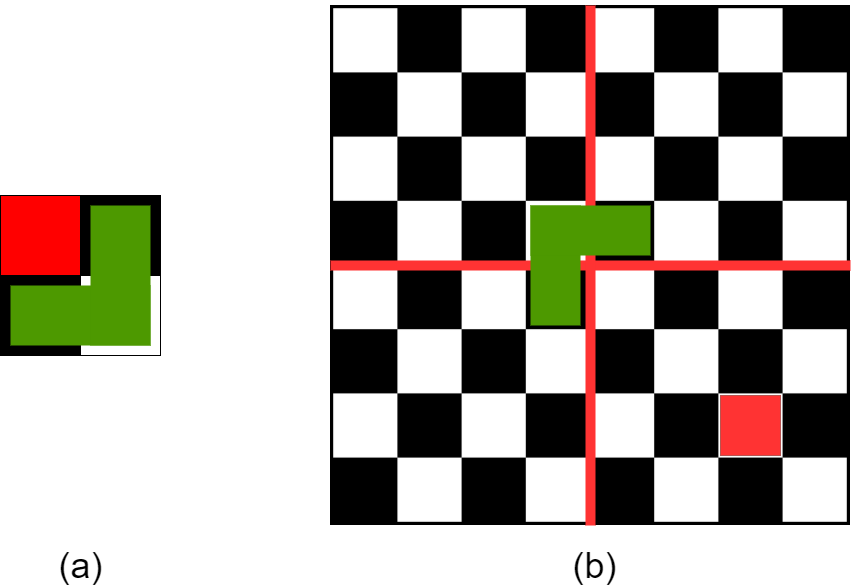
\includegraphics[width=0.5\textwidth]{Q2.png}
\caption{(a) Base case of a 2x2 tile with one missing square(in red). Place an $l-tile$ covering the other 3 tiles(in green). (b) A general case when one quadrant has missing tile. Place an $l-tile$ covering other quadrants, acting as missing tile for that quadrant, call $\proc{FillTiles}$ for all quadrants.}
\end{center}
\end{figure}
\item PSEUDO-CODE for Tile Filling Problem:
    
    \begin{codebox}
    \Procname{$\proc{FillTiles}(A(b), missingPoint, answerList)$}
    \li \textbf{Base case: if} $b=1$
    \li \quad 2x2 board. $answerList \leftarrow$ Add $l-tile$ of remaining 3 points
    \li $Q \leftarrow$ Quadrant of $missingPoint$
    \li $(Q_a, Q_b, Q_c) \leftarrow \{Q_{UL}, Q_{UR}, Q_{LL}, Q_{LR}\} - Q$
    \li $newTile \leftarrow l-tile$ of 3 adjecent points in $(Q_a, Q_b, Q_c)$
    \li $answerList \leftarrow$ Add $newTile$ 
    \li $(P_{UL}, P_{UR}, P_{LL}, P_{LR})\leftarrow$ $3$ points in $newTile$ and $missingPoint$\\ 
    \quad\quad\quad\quad\quad\quad\quad\quad\quad
    corresponding to $(Q_{UL}, Q_{UR}, Q_{LL}, Q_{LR})$
    \li $\proc{FillTiles}(\textsc{UpperLeft}(A)(b-1), P_{UL}, answerList)$
    \li $\proc{FillTiles}(\textsc{UpperRight}(A)(b-1), P_{UR}, answerList)$
    \li $\proc{FillTiles}(\textsc{LowerLeft}(A)(b-1), P_{LL}, answerList)$
    \li $\proc{FillTiles}(\textsc{LowerRight}(A)(b-1), P_{LR}, answerList)$
    \end{codebox}
\newpage
\item 
We can find the quadrant of any point in $\Theta(1)$ operations by comparing the quadrant bounds with the point. Thus lines $1-7$ will take $\Theta(1)$ time.\\
Lines $8-11$ each will take $T(b-1)$ time as each quarant of $2^b$x$2^b$ board is of size $2^{b-1}$x$2^{b-1}$.

So have, $T(b) = 4T(b-1) + \Theta(1)$.\\
Let $2^b = n$. Thus, $b = \log_2(n)$\\
We have, $T(\log(n)) = 4T(\log(n)-1)+\Theta(1)$\\
$T(\log(n)) = 4T(\log(n/2))+\Theta(1)$\\
Let $T(\log(n)) = S(n)$\\
$S(n) = 4S(n/2)+\Theta(1)$\\

Let $a = 4$, $b=2$ and $f(n) = \Theta(1)$. Thus we have above equations of the form:
$T(n) = aT(n/b) + f(n)$ for large values of $n$.

We have $n^{\log_b a} = n^{\log_{2} 2} = n^2$. Also we have $f(n) = \Theta(1)$. Hence, by using Case 1 of Master's Theorem, we have
    \begin{equation}
        \begin{split}
           S(n) &= \Theta(n^2)\\
           T(\log(n)) &= \Theta(n^2)\\
           T(b) &= \Theta((2^b)^2)\\
           \mathbf{T(b)} &= \mathbf{\Theta(4^b)}
        \end{split}
    \end{equation}
\end{enumerate}

\newpage

\begin{problem}Why 5 in Median?\end{problem}
Recall the deterministic selection algorithm:
\begin{codebox}
\Procname{$\proc{Select}(A[1,\ldots,n], i)$}
\li Base case if $|A|<5$.
\li $p \gets \proc{MedianOfMedians}(A)$
\li $A_\ell,A_r,i_p \gets \proc{Partition}(A,p)$
\li \If $i_p=i$ \Return $A[i_p]$ 
\li \ElseIf $i_p<i$ \Return $\proc{Select}(A_r, i-i_p)$
\li \Else \Return $\proc{Select}(A_\ell,i_p-i)$ \End
\end{codebox}
\begin{codebox}
\Procname{$\proc{MedianOfMedians}(A[1\twodots n])$}
\li Divide $A$ into lists of 5 elements. If only one element, return it.\label{divideline}
\li Compute the median of each small list, store these medians in a new list $B$
\li $p\gets \proc{Select}(B,\lceil n/10 \rceil)$
\li \Return $p$
\end{codebox}
\begin{enumerate}
  \item
Suppose Line~\ref{divideline} of $\proc{MedianOfMedians}$
  divides $A$ into lists of 3 elements each instead of $5$ elements and
  line 3 is modified to pick the $\lceil n/6 \rceil$\textsuperscript{th} element.
  State an upper and lower bound on the size of $A_{\ell}$.  Be as precise as you can.
\item  
 Analyze the running time of $\proc{Select}$ under the 3-element version of 
  $\proc{MedianOfMedians}$.
\end{enumerate}
\hfill
   
\noindent \textbf{Ans.}
\begin{enumerate}
    \item If $\proc{MedianOfMedians}$ divides A into list of 3 elements, we  have $\lceil \frac{1}{2}\lceil n/3 \rceil\rceil$  columns out of which all except 2 has 2 numbers in it that are smaller than the selected median. Thus we have,
    $$2\left(\left\lceil \frac{1}{2}\lceil n/3 \rceil\right\rceil-2\right)$$
    elements that are smaller than the selected median.
    Thus there are atleast $\frac{n}{3} -4$ elements that are smaller than the selected median.
    Similarly there are atleast $\frac{n}{3} -4$ elements that are greater than the selected median.
    Thus upper limit of median is $(n-(\frac{n}{3} -4))$ = $\frac{2n}{3} +4$.\\
    Hence the size of $A_{\ell}$ can be between
    $$\left[\frac{n}{3} -4, \frac{2n}{3} +4\right]$$
    
    \item We have $S(n) = P(n)+S'(n)$\\
    Since max size of $A_{\ell} = \frac{2n}{3} +4$, for 3-element we have\\
    $S(n) = P(n)+S(\frac{2n}{3} +4)$\\
    Also we have $P(n) = S(\lceil n/3 \rceil) + O(n)$\\
    Thus, we have\\
    $S(n) = S(\lceil n/3 \rceil) + O(n)+S(\frac{2n}{3} +4)$
    
    \noindent \textbf{Hypothesis:} $S(n) = \Theta(n\log(n))$\\
    \textbf{Hypothesis-1:} $S(n) \geq \frac{1}{100}n\log(n)$\\
    \noindent Base case, 
    \begin{equation}
        \begin{split}
           S(20) &= S(7)+S(17)+3\\
           &= 44\\
           &\geq \frac{1}{100}(20*\log(20))
        \end{split}
    \end{equation}
    Thus base case holds.\\
    \noindent Let there be a positive integer $k$ such that the equation is valid for all $n \leq k$. Thus,
    $$ S(k) \geq \frac{1}{100}(k\log(k))$$
    
    \noindent Now, for $n=k+1$, we have
    \begin{equation}
        \begin{split}
           S(k+1) &= S(\lceil (k+1)/3 \rceil) + S\left(\frac{2(k+1)}{3} +4\right)+(k+1)\\
           &\geq S\left(\frac{k+1}{3}\right) + S\left(\frac{2(k+1)}{3}\right)+(k+1)\\
           &= \frac{1}{100}\left(\frac{k+1}{3}\right)\log\left(\frac{k+1}{3}\right) + \frac{1}{100}\left(\frac{2(k+1)}{3}\right)\log\left(\frac{2(k+1)}{3}\right)+(k+1)\\
           &\geq \frac{1}{100}\left(\frac{k+1}{3}\right)\left[3*\log(k+1)-3\log(3)\right] +(k+1)\\
           &= \frac{1}{100}(k+1)\log(k+1) +(k+1)\left[1-\frac{log(3)}{100}\right]\\
           &\geq \frac{1}{100}(k+1)\log(k+1)
        \end{split}
    \end{equation}
    Which is the required RHS. Thus we have
    $$\mathbf{S(n) = \Omega(n\log(n))}$$
    

\noindent \textbf{Hypothesis-2:} $S(n) \leq 100*(n-15)\log(n-15)$\\
\noindent Base case, 
    \begin{equation}
        \begin{split}
           S(20) &= S(7)+S(17)+20\\
           &= 44\\
           &\leq 100(5*\log(5))
        \end{split}
    \end{equation}
    Thus base case holds.\\
    \noindent Let there be a positive integer $k$ such that the equation is valid for all $n \leq k$. Thus,
    $$ S(k) \leq 100(k-15)\log(k-15)$$
    
    \noindent Now, for $n=k+1$, we have
    \begin{equation}
        \begin{split}
           S(k+1) &= S(\lceil (k+1)/3 \rceil) + S\left(\frac{2(k+1)}{3} +4\right)+(k+1)\\
           &\leq S\left(\frac{k+4}{3}\right) + S\left(\frac{2k+14}{3} \right)+(k+1)\\
           &= 100\left(\frac{k-41}{3}\right)\log\left(\frac{k-41}{3}\right) + 100\left(\frac{2k-31}{3}\right)\log\left(\frac{2k-31}{3}\right)+(k+1)\\
           &\leq 100\left(\frac{k-41}{3}\right)\log(k-41) + 100\left(\frac{2k-31}{3}\right)\log(k-15)\\
           &\quad +(k+1)-100\left(\frac{k-41}{3}+\sqrt{2}\frac{2k-31}{3}\right)\log(3)\\
           &\leq 100\left(\frac{k-41}{3}\right)\log(k-41) + 100\left(\frac{2k-31}{3}\right)\log(k-15)\\
           &\leq 100\left(\frac{k-41}{3}\right)\log(k-14) + 100\left(\frac{2k-31}{3}\right)\log(k-14)\\
           &\leq 100\left(\frac{k-41}{3}+\frac{2k-31}{3}\right)\log(k-14)\\
           &\leq 100(k-14)\log(k-14)\\
           &\leq 100((k+1)-15)\log((k+1)-15)
        \end{split}
    \end{equation}
    Which is the required RHS. Thus we have
    $$\mathbf{S(n) = O(n\log(n))}$$
    Since, we have $T(n) = \Omega(n\log(n))$ and $T(n) = O(n\log(n))$.
    Hence we can say,
    $$\mathbf{T(n) = \Theta(n\log(n))}$$
\end{enumerate}




\newpage

\begin{problem}Peaks\end{problem}
On a clear day, the shores of lake Zurich offer a sublime view of the alpine mountainscape.  Define the \emph{left alpine function}, denoted $a_{\ell}(s)$,
of a mountain scape $s$ as the total number of times that a peak is taller than one of its left neighboring peaks. The \emph{right alpine function}, $a_r(\cdot)$, is defined analogously. The alpine mountainscape $s$ below
has 8 peaks, $a_\ell = 19$, the contribution of each peak is listed below the building.

\begin{center}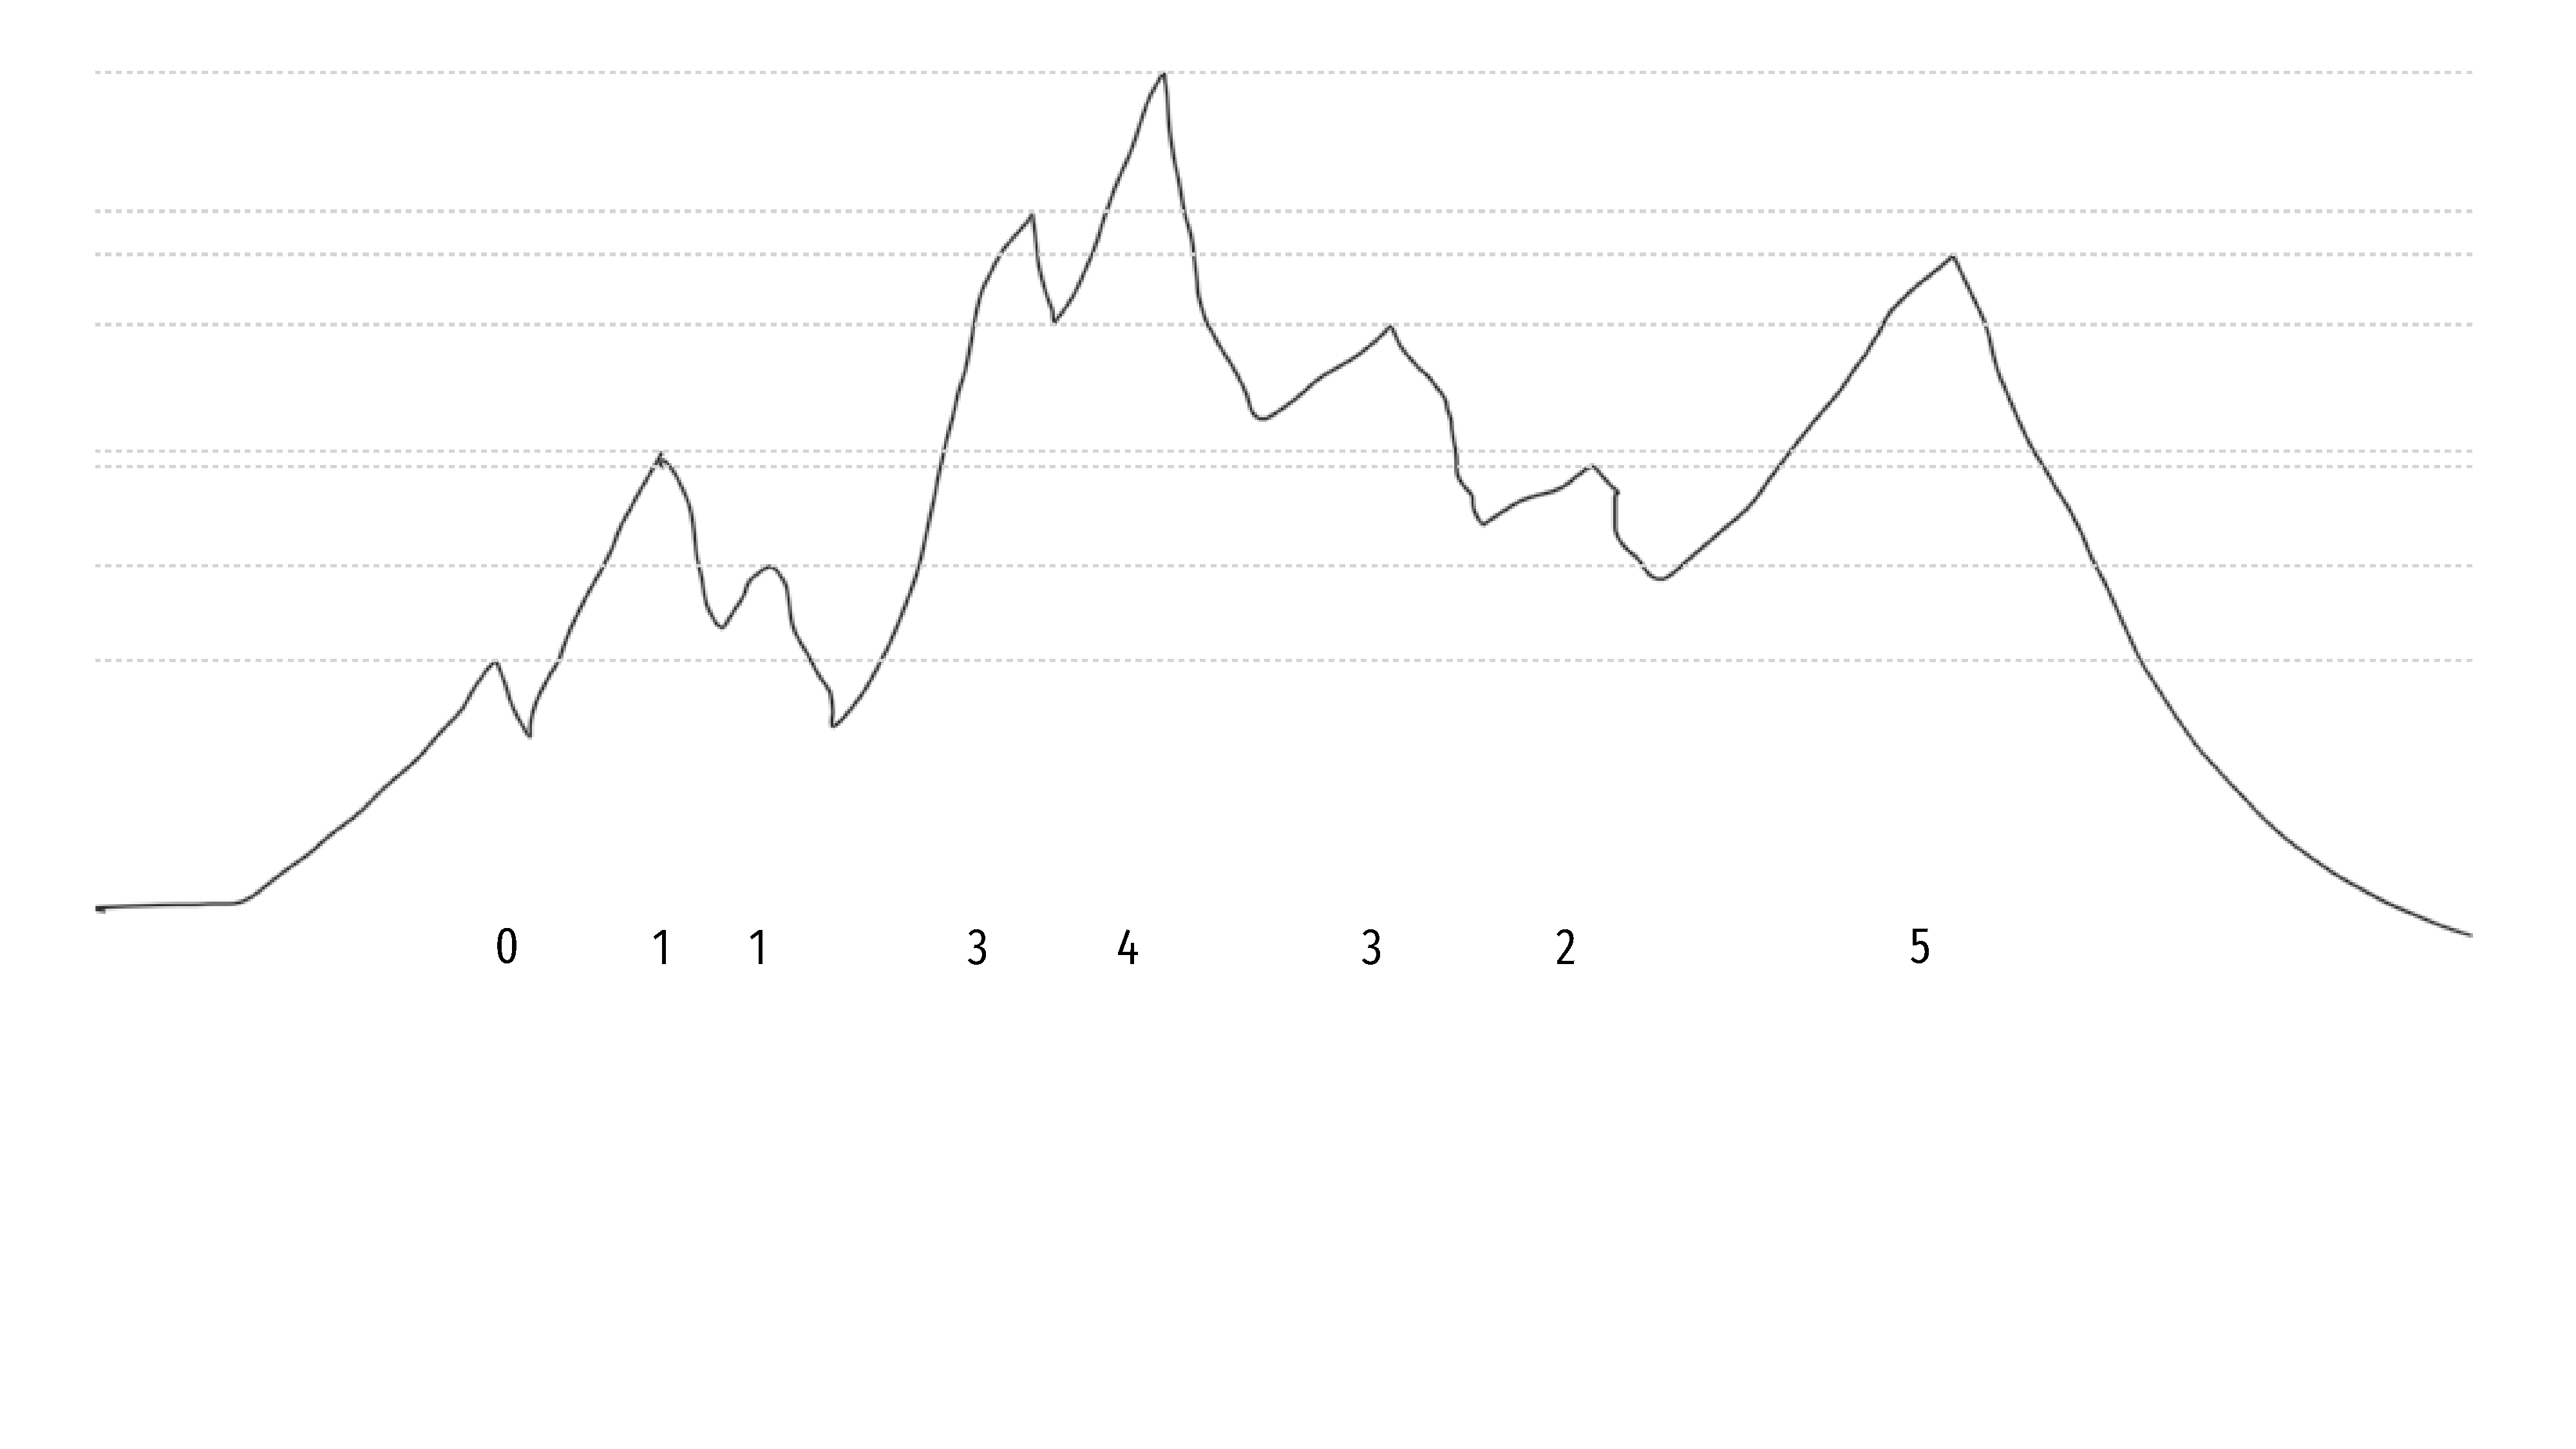
\includegraphics[scale=0.2]{mountains}\end{center}

Design and analyze a divide and conquer algorithm that computes both the left and right alpine functions of a mountainscape $s$ with $n$ peaks. The input $A[1,\ldots, n]$ consists of the heights of each peak in left to right order; assume all peaks have unique heights. Your solution should have a running time of $\Theta(n \log n)$ and should include an analysis of the running time.


\hfill
   
\noindent \textbf{Ans.}

Left alpine function($a_\ell$) of a mountain scape is the total number of times a peak is taller than peaks on its left. Thus for any given peak, its contribution to ($a_\ell$) can be found by counting the number of peaks smaller than itself that are on its left. We can count the number of peaks on the left smaller than the current peak by modifying the MergeSort algorithm. We can similarly calculate the right alpine function($a_r$).

In mergesort algorithm, we have a $leftArray$ and a $rightArray$. The current pointer position in $leftArray$ denotes the number of elements which are smaller than the current values of $leftIndex$ and $rightIndex$. Thus, adding the $leftIndex$ value everytime current value of $rightArray$ is less than current $leftArray$ will give the left alpine function. Similar calculation can be done for right alpine function as well.

\newpage
\noindent PSEUDO-CODE to calculate Alpine Functions:

    \begin{codebox}
    \Procname{$\proc{GetAlpineFunctions}(A[1,..,n])$}
    \li $a_\ell, a_r \leftarrow \{0, 0\}$
    \li $\proc{ModifiedMergeSort}(A, 0, n, \{a_\ell, a_r\})$
    \li \textbf{return} $\{a_\ell, a_r\}$
    \end{codebox}
    
    \begin{codebox}
    \Procname{$\proc{ModifiedMergeSort}(A[1,..,n], left, right, \{a_\ell, a_r\})$}
    \li \textbf{if} $left<right$
    \li \quad $mid \leftarrow \left\lfloor\frac{left+right}{2}\right\rfloor$
    \li \quad $\proc{ModifiedMergeSort}(A, left, mid, \{a_\ell, a_r\})$
    \li \quad $\proc{ModifiedMergeSort}(A, mid+1, right, \{a_\ell, a_r\})$
    \li \quad $\proc{Merge}(A, left, mid, right, \{a_\ell, a_r\})$
    \end{codebox}
    
    \begin{codebox}
    \Procname{$\proc{Merge}(A[1,..,n], left, mid, right, \{a_\ell, a_r\})$}
    \li $totLeft, totRight \leftarrow \{mid-left+1, right-mid\}$
    \li $LeftArray, RightArray \leftarrow \{A[left, .. , mid], A[mid+1, .. , right]\}$
    \li $\ell, r \leftarrow \{0, 0\}$
    \li \textbf{for} $k\leftarrow \{left, .. , right\}$
    \li \quad \textbf{if} $\ell>totLeft$
    \li \quad \quad $A[k] \leftarrow RightArray[r]$
    \li \quad \quad $r \leftarrow r+1$
    \li \quad \quad $a_\ell \leftarrow a_\ell + \ell-1$
    \li \quad \textbf{else if} $r>totRight$
    \li \quad \quad $A[k] \leftarrow LeftArray[\ell]$
    \li \quad \quad $\ell \leftarrow \ell+1$
    \li \quad \quad $a_r \leftarrow a_r + r-1$
    \li \quad \textbf{else if} $LeftArray[\ell]>RightArray[r]$
    \li \quad \quad $A[k] \leftarrow RightArray[r]$
    \li \quad \quad $r \leftarrow r+1$
    \li \quad \quad $a_\ell \leftarrow a_\ell + \ell-1$
    \li \quad \textbf{else}
    \li \quad \quad $A[k] \leftarrow LeftArray[\ell]$
    \li \quad \quad $\ell \leftarrow \ell+1$
    \li \quad \quad $a_r \leftarrow a_r + r-1$
    \end{codebox}
\newpage
 Time Complexity analysis for $\proc{GetAlpineFunctions}$
 \begin{enumerate}
     \item $\proc{GetAlpineFunctions} = G(n)$ calls $\proc{ModifiedMergeSort} = S(n)$ thus $G(n) =  S(n)$.
     \item $\proc{ModifiedMergeSort}$ calls itself twice with half size and calls $\proc{Merge} = M(n)$ once. Thus, $S(n) = 2S(n/2)+M(n)$.
     \item Lines $1-3$ in $\proc{Merge}$ takes $\Theta(1)$ time. Line $4$ $for$ loop runs $n$ times. All the operations in $if-else$ lines $5-20$ will take $\Theta(1)$ for each iteration. Thus $M(n) = \Theta(n)$
     \item Thus we have $S(n) = 2S(n/2)+\Theta(n)$.\\
     Let $a = 2$, $b=2$ and $f(n) = \Theta(n)$. Thus we have above equations of the form:\\
     $S(n) = aS(n/b) + f(n)$ for large values of $n$.

    We have $n^{\log_b a} = n^{\log_{2} 2} = n^1 = n$. Also we have $f(n) = \Theta(n)$. 
    Hence, by using Case 2 of Master's Theorem, we have, $S(n) = \Theta(n\log(n))$.
    \item Since $G(n) = S(n)$
    $$\mathbf{G(n) = \Theta(n\log(n))}$$
    This is intuitive from the fact that $\proc{GetAlpineFunctions}$ itself is a modified MergeSort with just $\Theta(1)$ operations added to calculate $a_\ell$ and $a_r$.
 \end{enumerate}
\end{document}
